 \documentclass[write-up.tex]{subfiles}
 \begin{document}
\section{Development and Testing}
%Talk about how the equation for the smoothing kernel changed to remove 15/(pi h^6) cuz values were too small, redo volume and derivatives as well as do some tweaking to find optimum values.
\subsection{Boilerplate code}

The beginning of my implementation involved the boilerplate minimal code required for my graphics library SFML to be setup as well as including key libraries I will need throughout the project.
\lstset{language=C++,
                breaklines=true,
                basicstyle=\ttfamily,
                keywordstyle=\color{blue}\ttfamily,
                stringstyle=\color{red}\ttfamily,
                commentstyle=\color{green}\ttfamily,
                morecomment=[l][\color{magenta}]{\#}
}
\begin{lstlisting}

#include <SFML/System/Vector2.hpp>
#include <SFML/Graphics.hpp>
#include<iostream>
#include <algorithm>
#include<vector>
#include<cmath>
#include <omp.h>

int main()
{
    //Initialize SFML
    sf::RenderWindow window(sf::VideoMode(900, 900), "Smoothed Particle Hydrodynamics Simulation");
    window.setFramerateLimit(120);
    sf::View view = window.getDefaultView();
    sf::Vector2u window_size = window.getSize();

    while (window.isOpen())
    {
        sf::Event event;
        while (window.pollEvent(event))
        {
            if (event.type == sf::Event::Closed)
                window.close();
            if (event.type == sf::Event::Resized){
                sf::FloatRect visibleArea(0.f, 0.f, event.size.width, event.size.height);
                window.setView(sf::View(visibleArea));
            }
        }
        sf::Vector2u window_size = window.getSize();
        window.clear();
        window.display();
    }
    return 0;
}
\end{lstlisting}

\subsection{Particle initialization}
We can begin adding particles using instances of a Particle struct which stores the information each particle needs. This includes position and velocity vectors, the circular shape, local densities and pressures and their predicted position.

\begin{lstlisting}
struct particle{
    sf::CircleShape droplet{particle_radius};
    sf::Vector2f position{0.f, 0.f};
    sf::Vector2f velocity{0.f, 0.f};
    float local_density = 0.f;
    float local_pressure = 0.f;
    sf::Vector2f predicted_position{0.f, 0.f};
};
\end{lstlisting}

We initialize a dynamic array of these particles and place them in an orderly fashion at the start of the simulation, as well as set their colour to cyan.

\begin{lstlisting}
const int particle_num = 1600;
const float particle_mass = 1.f;
vector<particle> particles(particle_num);

void placeParticles(){
    int particlesPerRow = sqrt(particle_num);
    int particlesPerColumn = (particle_num - 1)/particlesPerRow + 1;
    int spacing = 2.5*particle_radius;
    for (int i = 0; i < particle_num; i++){
        particles[i].position.x = (i % particlesPerRow + particlesPerRow / 2.5f +0.5f) * spacing;
        particles[i].position.y = (i / particlesPerRow + particlesPerColumn / 2.5f +0.5f) * spacing;
        particles[i].droplet.setFillColor(sf::Color::Cyan);
    }
}

\end{lstlisting}

\begin{figure}
\centering
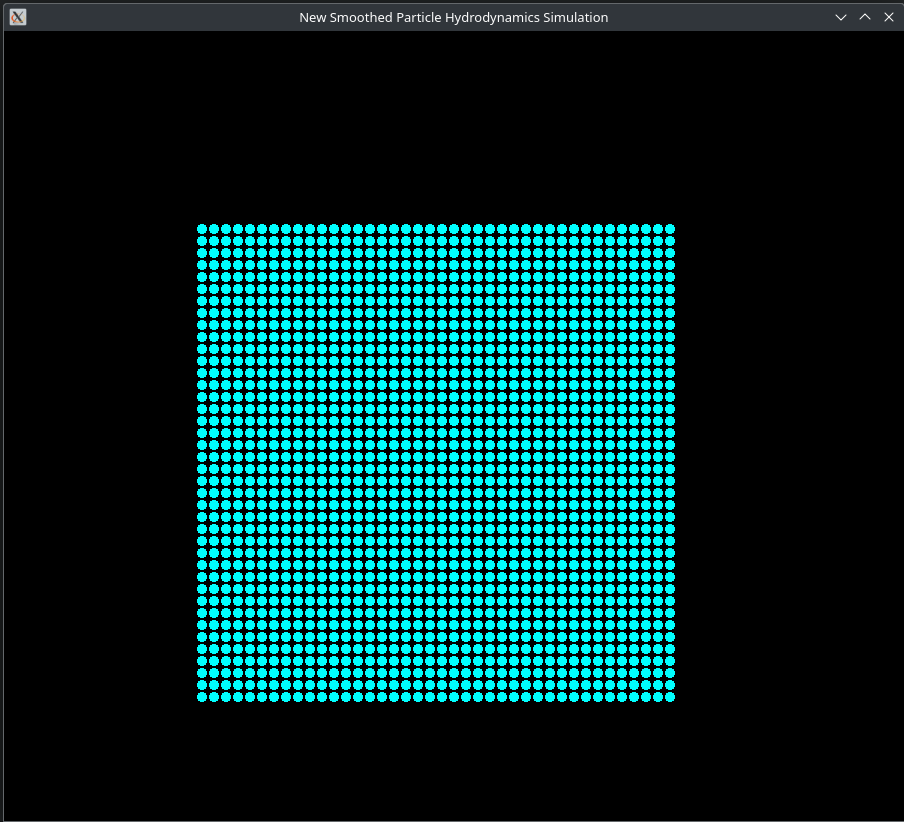
\includegraphics[width=15cm, height=15cm]{more_still_particles_19-05-24}
\caption{Particles placed in an orderly fashion on the screen}
\end{figure}

\newpage
\subsection{Simulation loop}
In order to calculate new positions of particles, we need to loop over them every step of the simulation to calculate its new position vector using its current velocity and acceleration vectors and multiplying by $dt$, our change in time per simulation step and then draw them. We can begin updating these by implementing gravity first.
\begin{lstlisting}
const float gravity = 9.81f;
const float dt = 1.f/60.f;

 void resolveGravity(int i){
    particles[i].velocity.y += gravity * dt
}
\end{lstlisting}

And within the simulation loop:
\begin{lstlisting}
for (int i = 0; i < particle_num; i++){
    resolveGravity(i);
    particles[i].position.x += particles[i].velocity.x * dt;
    particles[i].position.y += particles[i].velocity.y * dt;
    particles[i].droplet.setPosition(particles[i].position.x-particle_radius, particles[i].position.y-particle_radius);

    //Draw particles
    window.draw(particles[i].droplet);
\end{lstlisting}
This \href{https://youtube.com/shorts/FSuH_Cs1Qh4?feature=share}{video} shows the implementation of gravity but with no simulation border. This can be implmented with ease in the following manner:

\begin{lstlisting}
void resolveCollisions(int i, sf::Vector2u window_size){
    if (particles[i].position.x > window_size.x || particles[i].position.x < 0){
        particles[i].position.x = clamp((int)particles[i].position.x, 0, (int)window_size.x);
        particles[i].velocity.x *= -1 * collision_damping;
    }
    if (particles[i].position.y >= window_size.y || particles[i].position.y <= 0){
        particles[i].position.y = clamp((int)particles[i].position.y, 0, (int)window_size.y);
        particles[i].velocity.y *= -1 * collision_damping;
    }
}
\end{lstlisting}

I've also implemented a collision damping factor here to simulate the loss the energy upon collision with the simulation border. We now see that we can also successfully interact with the simulation by resizing our window, hitting one of the sucess criteria for this project. The video can be watched \href{https://youtube.com/shorts/wO0xUBSKVck?feature=share}{here}.
\subsection{Smoothing Kernel implementation}

As per the theoretical model, my preferred choice of smoothing kernel is $W_{\text{spiky}}(r, h)$ for large repulsion forces at small distances. In C++, this looks like the following:


 \end{document}
